% This is a model template for the solutions in computational science. You can find a very useful documentation for LaTeX in Finnish at ftp://ftp.funet.fi/pub/TeX/CTAN/info/lshort/finnish/ or in English at ftp://ftp.funet.fi/pub/TeX/CTAN/info/lshort/english/. The section List of mathematical symbols in Chapter 3 is especially useful for the typesetting of mathematical formulas.

% Compile the document to PDF by command 'pdflatex model.tex' in the terminal. The command must be run twice for the references in the text to be correct.

\documentclass[a4paper,11pt]{article}
\usepackage[utf8]{inputenc}
% This includes letters such as � and �
\usepackage[T1]{fontenc}
% Use here 'Finnish' for Finnish hyphenation. You may have to compile the code twice after the change. 
\usepackage[english]{babel}
\usepackage{graphicx}
% Some math stuff
\usepackage{amsmath,amsfonts,amssymb,amsbsy,commath,booktabs,hyperref}  
% This is just to include the urls
\usepackage{hyperref}
\usepackage[margin=2cm]{geometry}

\setlength{\parindent}{0mm}
\setlength{\parskip}{1.0\baselineskip}

\usepackage{listings}
\usepackage{color}

\definecolor{dkgreen}{rgb}{0,0.6,0}
\definecolor{gray}{rgb}{0.5,0.5,0.5}
\definecolor{mauve}{rgb}{0.58,0,0.82}

\lstset{frame=tb,
	language=Python,
	aboveskip=3mm,
	belowskip=3mm,
	showstringspaces=false,
	columns=flexible,
	basicstyle={\tiny\ttfamily},
	numbers=none,
	numberstyle=\tiny\color{gray},
	keywordstyle=\color{blue},
	commentstyle=\color{dkgreen},
	stringstyle=\color{mauve},
	breaklines=true,
	breakatwhitespace=true,
	tabsize=4
}

\begin{document}

\title{Becs-114.1100 Computational Science -- exercise round 4} % Replace the exercise round number
\author{Kunal Ghosh, 546247} % Replace with your name and student number
\maketitle
\section{Solution to Question 3}\label{prob3a}
\subsection{Evaluation of $\int_{0}^{2} \frac{1}{(1+x)}$}
\begin{lstlisting}
Analytical Integral is ln(3) =  1.09861228867
Numerical Integral is : 1.09861228867
Error is 2.22044604925e-16
1.3333333333
1.1666666667 1.1111111111
1.1166666667 1.1000000000 1.0992592593
1.1032106782 1.0987253487 1.0986403720 1.0986305484
1.0997677016 1.0986200427 1.0986130223 1.0986125882 1.0986125177
1.0989015152 1.0986127864 1.0986123026 1.0986122912 1.0986122900 1.0986122898
1.0986846188 1.0986123200 1.0986122889 1.0986122887 1.0986122887 1.0986122887 1.0986122887
1.0986303727 1.0986122906 1.0986122887 1.0986122887 1.0986122887 1.0986122887 1.0986122887 1.0986122887
1.0986168098 1.0986122888 1.0986122887 1.0986122887 1.0986122887 1.0986122887 1.0986122887 1.0986122887 1.0986122887
\end{lstlisting}

\subsection{Evaluation of $\int_{0}^{1} e^x$}
\begin{lstlisting}
Analytical Integral is e^1 - 1 =  1.71828182846
Numerical Integral is 1.71828182846
Error is 2.22044604925e-16
1.8591409142
1.7539310925 1.7188611519
1.7272219046 1.7183188419 1.7182826879
1.7205185922 1.7182841547 1.7182818422 1.7182818288
1.7188411286 1.7182819741 1.7182818287 1.7182818285 1.7182818285
1.7184216603 1.7182818376 1.7182818285 1.7182818285 1.7182818285 1.7182818285
1.7183167869 1.7182818290 1.7182818285 1.7182818285 1.7182818285 1.7182818285 1.7182818285
1.7182905681 1.7182818285 1.7182818285 1.7182818285 1.7182818285 1.7182818285 1.7182818285 1.7182818285
1.7182840134 1.7182818285 1.7182818285 1.7182818285 1.7182818285 1.7182818285 1.7182818285 1.7182818285 1.7182818285

\end{lstlisting}


\subsection{Evaluation of $\int_{0}^{1} sqrt(x)$}
\begin{lstlisting}
Analytical Integral is ln(3) =  0.666666666667
Numerical Integral is 0.666649928319
Error is 1.67383479868e-05
0.5000000000
0.6035533906 0.6380711875
0.6432830462 0.6565262648 0.6577566033
0.6581302216 0.6630792801 0.6635161478 0.6636075691
0.6635811969 0.6653981886 0.6655527825 0.6655851101 0.6655928651
0.6655589363 0.6662181827 0.6662728490 0.6662842786 0.6662870205 0.6662876990
0.6662708114 0.6665081031 0.6665274311 0.6665314721 0.6665324415 0.6665326814 0.6665327412
0.6665256573 0.6666106059 0.6666174395 0.6666188682 0.6666192109 0.6666192957 0.6666193169 0.6666193221
0.6666165490 0.6666468462 0.6666492622 0.6666497673 0.6666498885 0.6666499185 0.6666499260 0.6666499279 0.6666499283
\end{lstlisting}

Romberg's method expects that the integrand's derivative be defined at all points within the integrating limits. This pre-requisite is violated by the last function since its not differentiable at 0 and that's the reason Romberg's method doesn't perform as well in that case.

The corresponding python code can be found at \ref{code:problem3a}
 
\section{Solution to Question 5}\label{prob3b}
	
\begin{figure}[ht]
	\center
	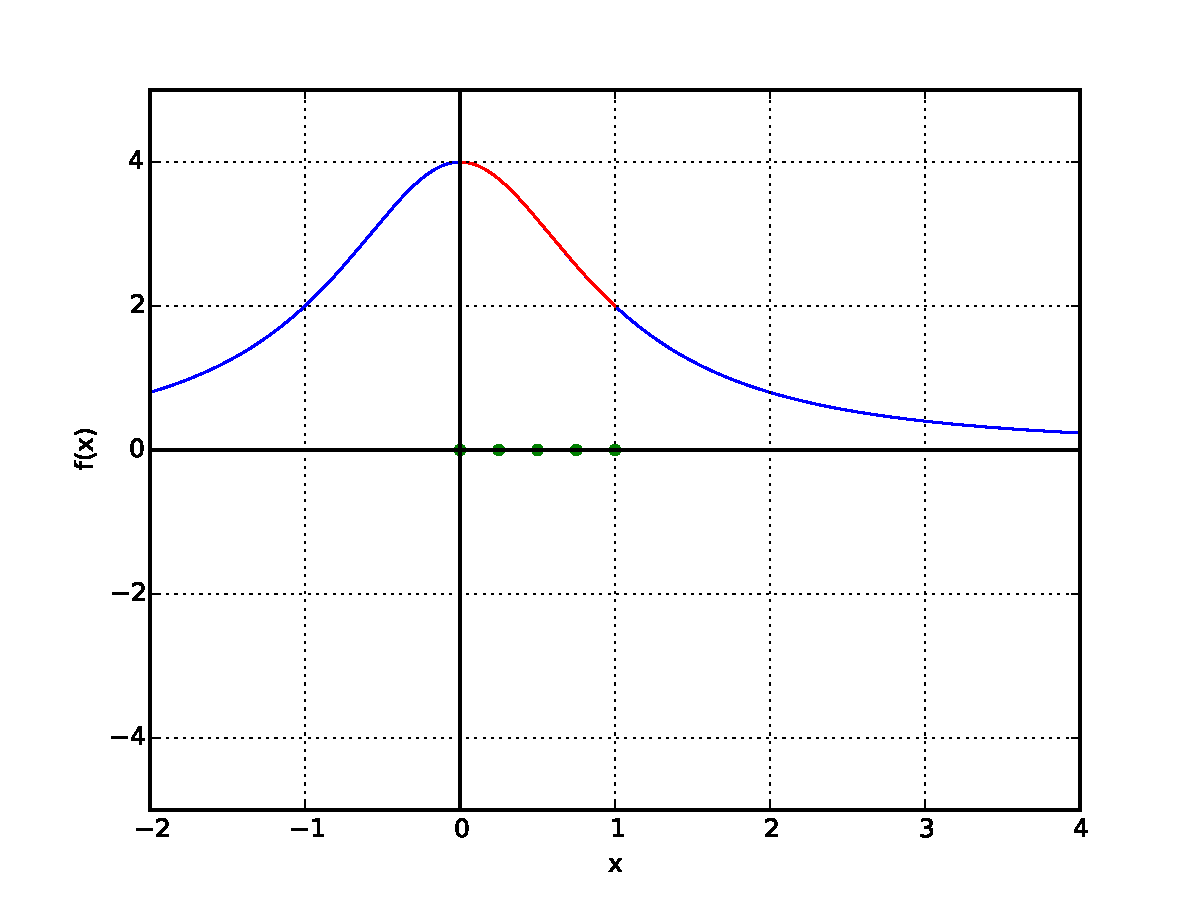
\includegraphics[scale=0.45]{ex5_fig1.pdf}
    \caption{Plot showing the actual curve of $\frac{4}{1+x^2}$ the red portion is the interval we are interested in integrating and the green points are the subdivisions generated by the adaptive simpson's method}
	\label{fig:fig1}
\end{figure}
for the first function the c values ( points of sub-division ) and the final integral are as follows:
\begin{lstlisting}
c=0.5
c=0.25
c=0.75
Numerical Integral by adaptive simpson's method: 3.14159250246
\end{lstlisting}

\begin{figure}[ht]
	\center
	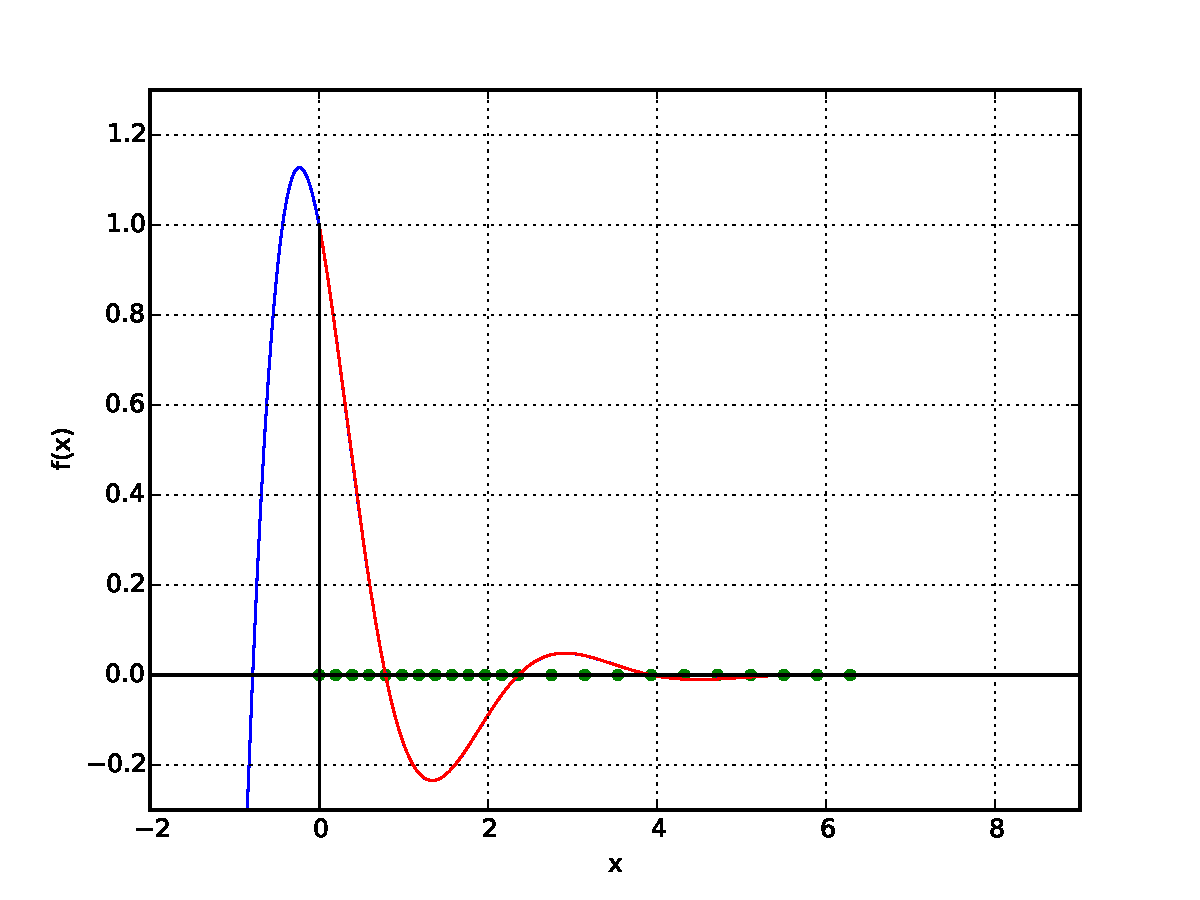
\includegraphics[scale=0.45]{ex5_fig2.pdf}
    \caption{Plot showing the actual curve of $\frac{cos(2x)}{e^x}$ the red portion is the interval we are interested in integrating and the green points are the subdivisions generated by the adaptive simpson's method}
	\label{fig:err1}
\end{figure}
for the second function the c values ( points of sub-division ) and the final integral are as follows:
\begin{lstlisting}
c=3.14159265359
c=1.57079632679
c=0.785398163397
c=0.392699081699
c=0.196349540849
c=0.589048622548
c=1.1780972451
c=0.981747704247
c=1.37444678595
c=2.35619449019
c=1.96349540849
c=1.76714586764
c=2.15984494934
c=2.74889357189
c=4.71238898038
c=3.92699081699
c=3.53429173529
c=4.31968989869
c=5.49778714378
c=5.10508806208
c=5.89048622548
Numerical Integral by adaptive simpson's method: 0.199622311724
\end{lstlisting}


	
In the two plots, the adaptive simpson's method automatically puts in more points in sub intervals where the integrand behaves like a higher order function and fewer points in the interval where the function behaves like a relatively lower order function. This is quite evident in the second plot where there are more intervals on the left portion of the integrand and fewer points on the right portion. Also a similar behavior is exhibited in the first graph where the integrand behaves like a lower order function in the integrating interval and the adaptive simpson's method puts fewer intervals.

The corresponding python code can be found at \ref{code:problem3b}
\clearpage


\section{Appendix A}\label{code:problem3a}
Python source code for \ref{prob3a}.
{\footnotesize
\begin{lstlisting}

from __future__ import division
import numpy as np

def recursive_trapezoid(n,R,f,a,b):
    '''
    Computes the integral evaluation using the recursive trapezoid rule.
    The function actually evaluates R(n,m) but since m is 0 for us to 
    prefer trapezoid rule, we don't accept that as an input.
    It accepts the function 'f' we are evaluating.
    returns R(n,0) added to R.

    The base case of this recursive this function is R(0,0) which
    is assumed to have already been inserted into the dictionary R
    that's why it is not added here.
    '''
    retVal = -1
    if (n,0) in R.keys():
        retVal = R[(n,0)]
    elif n == 0:
        retVal = 0.5 * (b-a) * (f(a) + f(b))
    else:
        h = (b-a) * (0.5 ** n)
        retVal = 0.5 * recursive_trapezoid(n-1, R, f, a, b) + h * sum([ f(a+(2*k-1)*h) for k in xrange(1,(2**(n-1))+1)])
    return retVal

def get_R(n, m, R, f, a, b):
    '''
    This function computes and returns the value of R with R(n,m) added to it.
    It expects the old R as an input and also the function we are evaluating
    '''
    retVal = -1
    if (n,m) in R.keys():
        retVal = R[(n,m)]
    elif m == 0:
        # call recursive trapezoidal function
        retVal = recursive_trapezoid(n,R,f,a,b)
    else:
        retVal = get_R(n,m-1,R,f,a,b) + (1.0/((4**m)-1)) * (get_R(n,m-1,R,f,a,b) - get_R(n-1,m-1,R,f,a,b))
    return retVal
        
def integrate(f,a,b,nrows):
    # The R "matrix" which would store the values computed from trapezoidal and
    # Romberg's algorithm
    # This is implemented as a dictionary which stores a tuple (n,m) as the key
    # and the corresponding R(n,m) evaluation as the value against the (n,m) key
    R = {}
    rows = nrows
    for i in range(rows):
        for j in range(i+1):
            R[(i,j)] = get_R(i,j,R,f,a,b)
    return R[i,j], R

def printR(R, n):
    for i in range(rows):
        for j in range(i+1):
            print("{0:.10f}".format(R[(i,j)])),
        print
    print

if __name__ == '__main__':
    rows = 9
    #---------function 
    print("Analytical Integral is ln(3) = "),
    Actual = 1.0986122886681098
    print(Actual)
    f = lambda x: 1 / (1+x)
    a = 0
    b = 2
    integral, R = integrate(f,a,b,rows)
    print "Numerical Integral is :",integral
    print("Error is {}".format(abs(Actual-integral)))
    printR(R,rows)
    #---------function 2
    print("Analytical Integral is e^1 - 1 = "),
    Actual = 1.718281828459045
    print(Actual)
    f = lambda x: np.e ** x 
    a = 0
    b = 1
    integral, R = integrate(f,a,b,rows)
    print "Numerical Integral is", integral
    print("Error is {}".format(abs(Actual-integral)))
    printR(R,rows)
    #---------function 3
    print("Analytical Integral is 2/3 = "),
    Actual = 0.6666666666666666
    print(Actual)
    f = lambda x: np.sqrt(x) 
    a = 0
    b = 1
    integral, R = integrate(f,a,b,rows)
    print "Numerical Integral is", integral
    print("Error is {}".format(abs(Actual-integral)))
    printR(R,rows)

\end{lstlisting}
}

\clearpage
\section{Appendix B}\label{code:problem3b}
Python source code for \ref{prob3b}.
{\footnotesize
\begin{lstlisting}

from __future__ import division
import numpy as np
import pylab as pl

def S(f,a,b):
    # Implement's the Simpson's method
    h = abs(b-a)
    c = (a+b)/2.0
    return (h/6.0) * (f(a) + 4*f(c) + f(b))

def adaptive_simpson(f,a,b,e,level_max):
    retVal = None
    c = (a+b)/2.0
    s1 = S(f,a,b)
    s2 = S(f,a,c) + S(f,c,b)
    err = (1/15.0)*(abs(s2 - s1))
    print "c={}".format(c)
    inpts.append(a)
    inpts.append(b)
    inpts.append(c)
    if level_max == 0 or err < e :
        # base case 
        # print " a={}, b={}, c={}, s1={}, s2={}, level={}".format(a,b,c,s1,s2,level_max)
        retVal = s2
    elif  err > e:
        # sub divide into left and right
        left = adaptive_simpson(f,a,c,e/2.0,level_max -1)
        right = adaptive_simpson(f,c,b,e/2.0,level_max -1)
        retVal = left + right
    return retVal

if __name__ == '__main__':
    # call adaptive simpson's for
    e = 0.5 * 10**(-4)
    level_max = 30
    # function 1
    f = lambda x: 4.0/(1 + x**2)
    a = 0
    b = 1
    inpts = [] # intervals
    result = adaptive_simpson(f,a,b,e,level_max)
    print("Numerical Integral by adaptive simpson's method: {}".format(result))

    xmin,xmax = int(a-2),int(b+2)+1 # for plots
    ymin,ymax = -5,5 # for plots
    x = np.linspace(xmin,xmax,1000)#floor and ceil used incase a and b are not ints
    x_interest = np.linspace(a,b,1000)
    pl.plot(x,f(x))
    pl.plot(x_interest, f(x_interest),color='red')
    # plotting axes
    pl.plot(range(xmin,xmax+1), 0*np.arange(xmin,xmax+1), color='black')
    pl.plot(0*np.arange(ymin,ymax+1), range(ymin,ymax+1), color='black')
    pl.scatter(inpts, [0 for _ in inpts], color="green")
    pl.plot()
    pl.xlabel("x")
    pl.ylabel("f(x)")
    pl.xlim(xmin,xmax)
    pl.ylim(ymin,ymax)
    pl.grid()
    pl.savefig("ex5_fig1.pdf")
    pl.show()
    
    # function 2
    f = lambda x: np.cos(2.0*x)/(np.e ** x)
    a = 0
    b = 2*np.pi
    inpts = [] # intervals
    result = adaptive_simpson(f,a,b,e,level_max)
    print("Numerical Integral by adaptive simpson's method: {}".format(result))

    xmin,xmax = int(a-2),int(b+2)+1 # for plots
    ymin,ymax = -0.3,1.3 # for plots
    x = np.linspace(xmin,xmax,1000)#floor and ceil used incase a and b are not ints
    x_interest = np.linspace(a,b,1000)
    pl.xlabel("x")
    pl.xlim(xmin,xmax)
    pl.ylim(ymin,ymax)
    pl.grid()
    pl.ylabel("f(x)")
    pl.plot(x,f(x))
    pl.plot(x_interest, f(x_interest),color='red')
    # plotting axes
    pl.plot(range(xmin,xmax+1), 0*np.arange(xmin,xmax+1), color='black')
    pl.plot(0*np.arange(int(ymin)-1,int(ymax)+1), range(int(ymin)-1,int(ymax)+1), color='black')
    pl.scatter(inpts, [0 for _ in inpts], color="green")
    pl.savefig("ex5_fig2.pdf")
    pl.show()

\end{lstlisting}
}

\end{document}

